\documentclass{article}
\usepackage{amsthm}
\usepackage{amsmath}
\usepackage{graphicx}
\usepackage{tikz}
\usepackage{wasysym}

\newtheorem{problem}{Problem}

\begin{document}
\title{Graph Traversal}
\author{Henry Z. Lo}
\maketitle

\section{Traversal Algorithms}
\subsection{Breadth first search}
\subsubsection{Description}
Breadth-first search traverses nodes level by level.  From the start node, the algorithm first visits its neighbors, then neighbors of neighbors, and so on.

As an example, consider the graph of New England in figure \ref{ne}.  If the algorithm traverses clockwise, and we begin at MA, then the order of visitation will be \texttt{MA->VT->NH->RI->CT->ME}.  

\begin{figure}
\centering
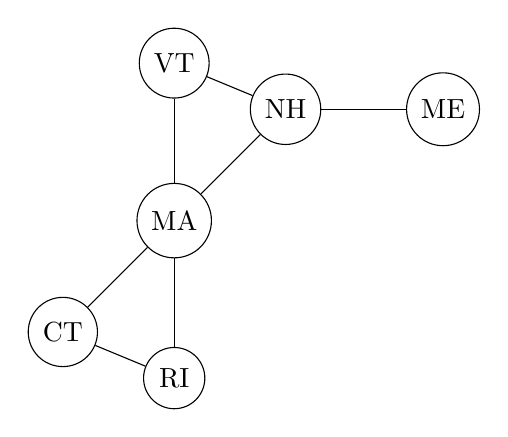
\begin{tikzpicture}[main node/.style={draw, circle}, node distance=2cm]
\node[main node]             (ma) {MA};
\node[main node, below of=ma] (ri) {RI};
\node[main node, below left of=ma] (ct) {CT};
\node[main node, above of=ma] (vt) {VT};
\node[main node, above right of=ma] (nh) {NH};
\node[main node, right of=nh] (me) {ME};
\path
(ma) edge node {} (ct)
     edge node {} (vt)
     edge node {} (nh)
     edge node {} (ri)
(vt) edge node {} (nh)
(me) edge node {} (nh)
(ct) edge node {} (ri);
\end{tikzpicture}
\caption{Graph representing the states in New England. \label{ne}}
\end{figure}

The algorithm must avoid cycles, and so it can be thought of as traversing the spanning tree in figure \ref{ne-span}.  Note that the tree is relatively balanced, and is constructed level by level.

\begin{figure}
\centering
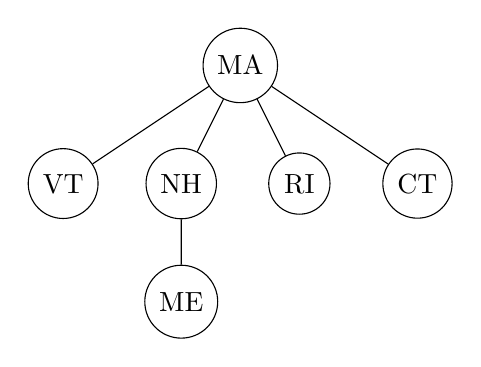
\begin{tikzpicture}[main node/.style={draw, circle}, node distance=2cm]
\node [main node] {MA}
	child{ node [main node] {VT}}
	child{ node [main node] {NH}
		child{ node [main node] {ME}}}
	child{ node [main node] {RI}}
	child{ node [main node] {CT}};
\end{tikzpicture}
\caption{Breadth-first spanning tree of New England. \label{ne-span}}
\end{figure}

\subsubsection{Algorithm}

The algorithm makes use a queue, which keeps track of which elements to visit next.  The LIFO structure of the queue guarantees that elements closest to the start are visited before elements further away.

The algorithm:
\begin{verbatim}
  BFS(start, target):
    q = new Queue<Node>
    visited = new Set<Node>
    q.enqueue(start)
    visited.add(start)

    while q not empty:
      node = q.dequeue()
      if node==target:
        return target
      for all neighbors n of node:
        if !visited.contains(n):
          q.enqueue(n)
          visited.add(n)
    return null
\end{verbatim}

The algorithm is $O(V)$, as is depth-first search, since in the worst case it visits all nodes (e.g. when the element we are looking for doesn't exist).

\subsubsection{Discussion}
While running, the queue in BFS may need to store many nodes at the same time (at worst, $O(V)$).  This is particularly worse for "wide" trees, but "deep" trees are OK.

Breadth first search is useful for finding the shortest path (in terms of number of edges) between two elements.  Note that in order to get an actual path, we need to keep track of the "parents" of each node in the spanning tree.

\subsection{Depth first search}
\subsubsection{Description}
Unlike BFS, DFS travels down a path until it can go no further, then backtracks until it finds other paths.  It does this until all nodes are traversed

For the New England graph, DFS will yield \texttt{MA->VT->NH->ME->RI->CT}, if we go clockwise from MA.  The spanning tree induced by this algorithm is shown in figure \ref{ne-dfs-span}.  DFS spanning trees tend to be very long, and can be very unbalanced.

\begin{figure}
\centering
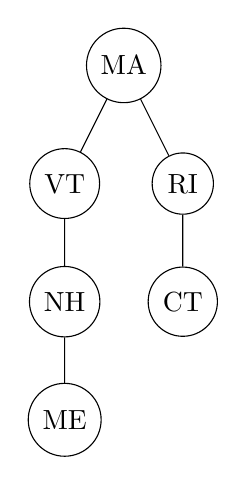
\begin{tikzpicture}[main node/.style={draw, circle}, node distance=2cm]
\node [main node] {MA}
	child{ node [main node] {VT}
		child{ node [main node] {NH}
			child{ node [main node] {ME}}}}
	child{ node [main node] {RI}
		child{ node [main node] {CT}}};
\end{tikzpicture}
\caption{Depth-first spanning tree of New England. \label{ne-dfs-span}}
\end{figure}

\subsubsection{Algorithm}

The algorithm makes use of a stack to keep track of its current path.  The LIFO structure of the queue guarantees that elements closest to the start are visited before elements further away.

The recursive algorithm:
\begin{verbatim}
  visited = new Set<Node>
  DFS(start, target):
    visited.add(start)
    for each neighbor n of start:
        if not visited
          visited.add(n)
          result = DFS(n)
          if result not null
            return result
    return null
\end{verbatim}

As with most recursive algorithms, we can also just use a stack:
\begin{verbatim}
  visited = new Set<Node>
  DFS(start, target):
    s = new Stack<Node>
    s.push(start)
    visited.add(start)

    while s not empty:
      node = s.pop()
      if node==target:
        return target
      for each neighbor n of node:
        if not visited
          visited.add(n)
          s.push(node)
    return null
\end{verbatim}

\subsubsection{Discussion}
The DFS stack DFS will need to store the longest path in the graph, which may be up to $O(V)$.  This is alright for wide trees, but unable to cope with deep trees (or very large graphs, such as road networks).

Depth first traversal is used in memoization, artificial intelligence, and playing games, as we have seen.  Though it does not find the shortest path to its destination, it is useful when we want to get to a leaf as quickly as possible.  For example, in the minimax algorithm, we need to get to the leaves to recursively analyse a path.  The stack also provides a nice representation of the current path, which may be useful for some problems.

\section{Pathfinding Algorithms}
The pathfinding problem is to find the shortest path between a start and end node.  This can be done using BFS in unweighted graphs, but when we have weights, we must use an algorithm like Dijkstra's.  

\subsection{Dijkstra's algorithm}
\subsubsection{Description}
Dijkstra's algorithm can be used to find the shortest path from any node to all other nodes in a graph.  When we are just interested in one destination, we can stop the algorithm early.

The algorithm keeps track of a map, which stores the shortest path length to each node.

See figure \ref{dijkstra} for an example.  We follow the status of the map as we run Dijkstra's algorithm.

\begin{figure}
\includegraphics[width=\textwidth]{img/dijkstra.png}
\caption{Dijkstra's algorithm on a directed graph. Source node is $s$, and target is $t$. \label{dijkstra}}
\end{figure}

\begin{enumerate}
\item Initially, the source path is 0, and all other path lengths are infinite.
\begin{center}
\begin{tabular}{cccccc}
$s$ & $t$ & $x$ & $y$ & $z$ \\
\hline
0 & $\infty$ & $\infty$ & $\infty$ & $\infty$
\end{tabular}
\end{center}

\item The edges connecting to $s$ give us one way to get to $t$ and $y$.  We store these edge values as the current best possible way to get to these nodes.  After this, we are done with $s$.
\begin{center}
\begin{tabular}{cccccc}
$s$ & $t$ & $x$ & $y$ & $z$ \\
\hline
0 & 10 & $\infty$ & 5 & $\infty$
\end{tabular}
\end{center}

\item Now we pick the closest node, which is $s$, and look at its edges.  We look at the edges to $x$ and $z$.  Adding these edge weights to our current path length (5) gives us the total distance to these nodes.  Also, we note that we find a faster path to $t$, and overwrite the previous value for $t$ in our map.
\begin{center}
\begin{tabular}{cccccc}
$s$ & $t$ & $x$ & $y$ & $z$ \\
\hline
0 & 8 & 14 & 5 & 7
\end{tabular}
\end{center}

\item We then visit the next closest node $z$.  $z$ contains an edge to $s$, but that total path length is greater than the one stored, so we ignore it.  $z$ also leads to $x$; adding that edge weight gives a total path length of 13.  We store this, because it is closer than the previously stored 14 path.
\begin{center}
\begin{tabular}{cccccc}
$s$ & $t$ & $x$ & $y$ & $z$ \\
\hline
0 & 8 & 13 & 5 & 7
\end{tabular}
\end{center}

\item We then visit the next closest node $t$.  $t$ has an edge to $x$, with a total path weight of $9$.  We store this, and ignore the edge to $y$.
\begin{center}
\begin{tabular}{cccccc}
$s$ & $t$ & $x$ & $y$ & $z$ \\
\hline
0 & 8 & 9 & 5 & 7
\end{tabular}
\end{center}

\item Finally, we visit $x$.  There are no edges worth storing here, so we are done.

\end{enumerate}

\subsubsection{Algorithm}
The algorithm:
\begin{verbatim}
  Dijkstra(start, target):
    m = new Map<Node,Integer>
    unvisited = new Set<Node>
    for n in nodes:
      if n==start
        m[n] = 0
      else
        m[n] = infinity
      unvisited.add(n)
      
    while unvisited not empty:
      n1 = node in unvisited with minimum distance
      if n1==target:
        return m[n1]
      unvisited.remove(n1)
      for each neighbor n2 of n1:
        path_length = dist[n1] + weight of (n1,n2)
        if path_length < dist[n2]
          dist[n2] = path_length
\end{verbatim}

Note that in the worst case, the inner for loop must iterate over all edges \textit{in total}, not for each iteration of the outer loop.  The while loop runs until all nodes are visited, though it can end early.  A naive implementation of the minimum distance node statement will be $O(V)$.  Thus, the naive Dijkstra's algorithm is $O(E+V^2)$.

We can improve this runtime if we keep a priority queue of unvisited nodes, ranked by their path lengths.  This makes retrieving this node $O(1)$, and removing to be $O(\log n)$, improving the overall runtime to $O(E + V \log V)$.

\subsection{A* search}
\subsubsection{Description}
Dijkstra's algorithm picks the next node greedily based on proximity to the start node.  This leads to a "spreading" around the start node, like in breadth first search.

For example, see the graph in figure \ref{bos}.  If we want to get to the airport from Charlestown, Dijktra's algorithm would give the sequence:
\[
\mbox{Charlestown} \rightarrow \mbox{Somerville} \rightarrow \mbox{Cambridge} \rightarrow \mbox{Chelsea} \rightarrow \mbox{Everett} \rightarrow \mbox{Airport}
\]

We first try the routes to Cambridge, Somerville, and Everett through Chelsea, because they are closer to where we started.  This doesn't make much sense because these take us further away from the airport.

\begin{figure}
\centering
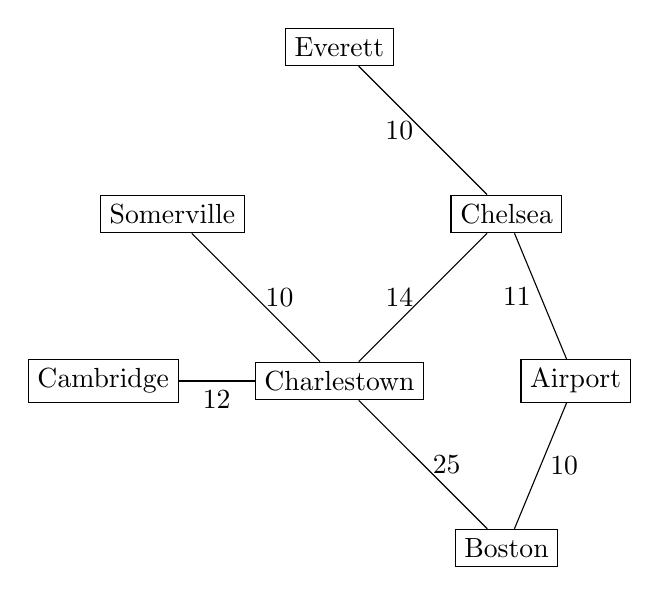
\begin{tikzpicture}[main node/.style={draw}, node distance=3cm]
\node[main node]                    (ct) {Charlestown};
\node[main node, above left of=ct]  (so) {Somerville};
\node[main node, left of=ct]        (ca) {Cambridge};
\node[main node, above right of=ct] (ch) {Chelsea};
\node[main node, above left of=ch]  (ev) {Everett};
\node[main node, below right of=ct] (bo) {Boston};
\node[main node, right of=ct]       (air) {Airport};
\path
(ct) edge [right] node {10} (so)
     edge [below] node {12} (ca)
     edge [left]  node {14} (ch)
     edge [right]  node {25} (bo)
(bo) edge [right] node {10} (air)
(air)edge [left] node {11} (ch)
(ch) edge [left] node {10} (ev);
\end{tikzpicture}
\caption{Graph representing some areas of Boston.  Edge weights represent driving times in minutes. \label{bos}}
\end{figure}


We can direct the search to the target if we have some kind of estimator for how close we are to it.  This function is called a heuristic.  A good distance for this type of problem is straight line driving time to the airport.  If we have this table of approximate times to the airport, we can use this in our search algorithm.

\begin{center}
\begin{tabular}{ccccc}
Cambridge & Somerville & Everett & Chelsea & Boston \\
\hline
30 & 28 & 20 & 14 & 12
\end{tabular}
\end{center}

We use these estimates of the driving time left by adding them to the time taken to get to each node.  This would result in the following map in Dijkstra's algorithm (we leave out Charlestown due to space).

\begin{center}
\begin{tabular}{c|cccccccc}
Step & Cambridge & Somerville & Everett & Chelsea & Boston & Airport \\
\hline
0 & $\infty$ & $\infty$ & $\infty$ & $\infty$ & $\infty$ & $\infty$ \\
1 & 12 + 30 & 10+28 & $\infty$ & 14+14 & 25+12 & $\infty$ \\
2 & 12 + 30 & 10+28 & $\infty$ & 14+14 & 25+12 & 25 \\
\end{tabular}
\end{center}

This modified Dijkstra's algorithm is called A* search.  A* gives the much more direct sequence:
\[
\mbox{Charlestown} \rightarrow \mbox{Chelsea} \rightarrow \mbox{Airport}
\]

\subsubsection{Algorithm}
The algorithm is exactly the same as Dijkstra's, except that we include calls the heuristic function $g$ to get the estimated driving time left:
\begin{verbatim}
  A*(start, target):
    m = new Map<Node,Integer>
    unvisited = new Set<Node>
    for n in nodes:
      if n==start
        m[n] = 0
      else
        m[n] = infinity
      unvisited.add(n)
      
    while unvisited not empty:
      n1 = node in unvisited with minimum distance
      if n1==target:
        return m[n1]
      unvisited.remove(n1)
      for each neighbor n2 of n1:
        path_length = dist[n1] + weight of (n1,n2) + g(n2)
        if path_length < dist[n2]
          dist[n2] = path_length
\end{verbatim}

Dijkstra's algorithm can be thought of a special case of A*, in which the heuristic function is always 0.

Choosing the heuristic depends on the problem domain.  In general, we want one that underestimates the actual cost to get to the goal (e.g. straight line driving time, or distance).

\end{document}